\begin{center}
    \begin{figure}[H]
        \centering

        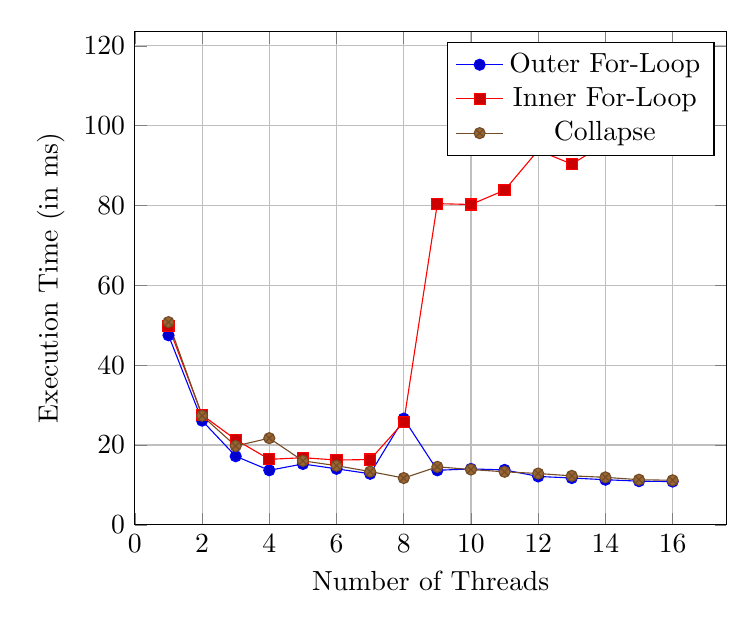
\begin{tikzpicture}
            \begin{axis}[
                title={},
                width=0.75\textwidth,
                xlabel={Number of Threads},
                ylabel={Execution Time (in ms)},
                xmin=0,
                ymin=0,
                grid=major
            ]
                \addplot coordinates {
                    (1,47.4856)(2,26.0906)(3,17.1762)(4,13.65)(5,15.2361)(6,14.0216)(7,12.7772)(8,26.5975)(9,13.65)(10,14.0004)(11,13.7465)(12,12.1108)(13,11.7167)(14,11.2901)(15,10.9296)(16,10.8207)
                };
                \addlegendentry{Outer For-Loop}

                \addplot coordinates {
                    (1,49.7317)(2,27.5263)(3,21.3296)(4,16.3962)(5,16.8052)(6,16.226)(7,16.3412)(8,25.7123)(9,80.4579)(10,80.2426)(11,83.8239)(12,93.8307)(13,90.3553)(14,95.5529)(15,112.304)(16,109.444)
                };
                \addlegendentry{Inner For-Loop}       

                \addplot coordinates {
                    (1,50.772)(2,27.3163)(3,19.7423)(4,21.7001)(5,16.0099)(6,14.8033)(7,13.3408)(8,11.7108)(9,14.5207)(10,13.8433)(11,13.274)(12,12.845)(13,12.2565)(14,11.8881)(15,11.2955)(16,11.1468)
                };
                \addlegendentry{Collapse}
            \end{axis}
        \end{tikzpicture}
        \caption{HSV Performance Tests dice\_large.png}
    \end{figure}
\end{center}